%%%%%%%%%%%%%%%%%%%%%%%%%%%%%%%%%
%  Figure subfigure template
%%%%%%%%%%%%%%%%%%%%%%%%%%%%%%%%%
\iffalse

\begin{figure}[ht]
  \centering
  \begin{subfigure}[b]{\textwidth}
    \centering
    \includegraphics[width=\textwidth]{}
    \caption{}
    \label{}
  \end{subfigure}
  \caption{}
  \label
\end{figure}

\fi



\chapter{Results} \label{cha:results}
TODO: Overview of results chapter.

% 800 Office woman

\iffalse
\begin{figure}[ht]
  \centering
  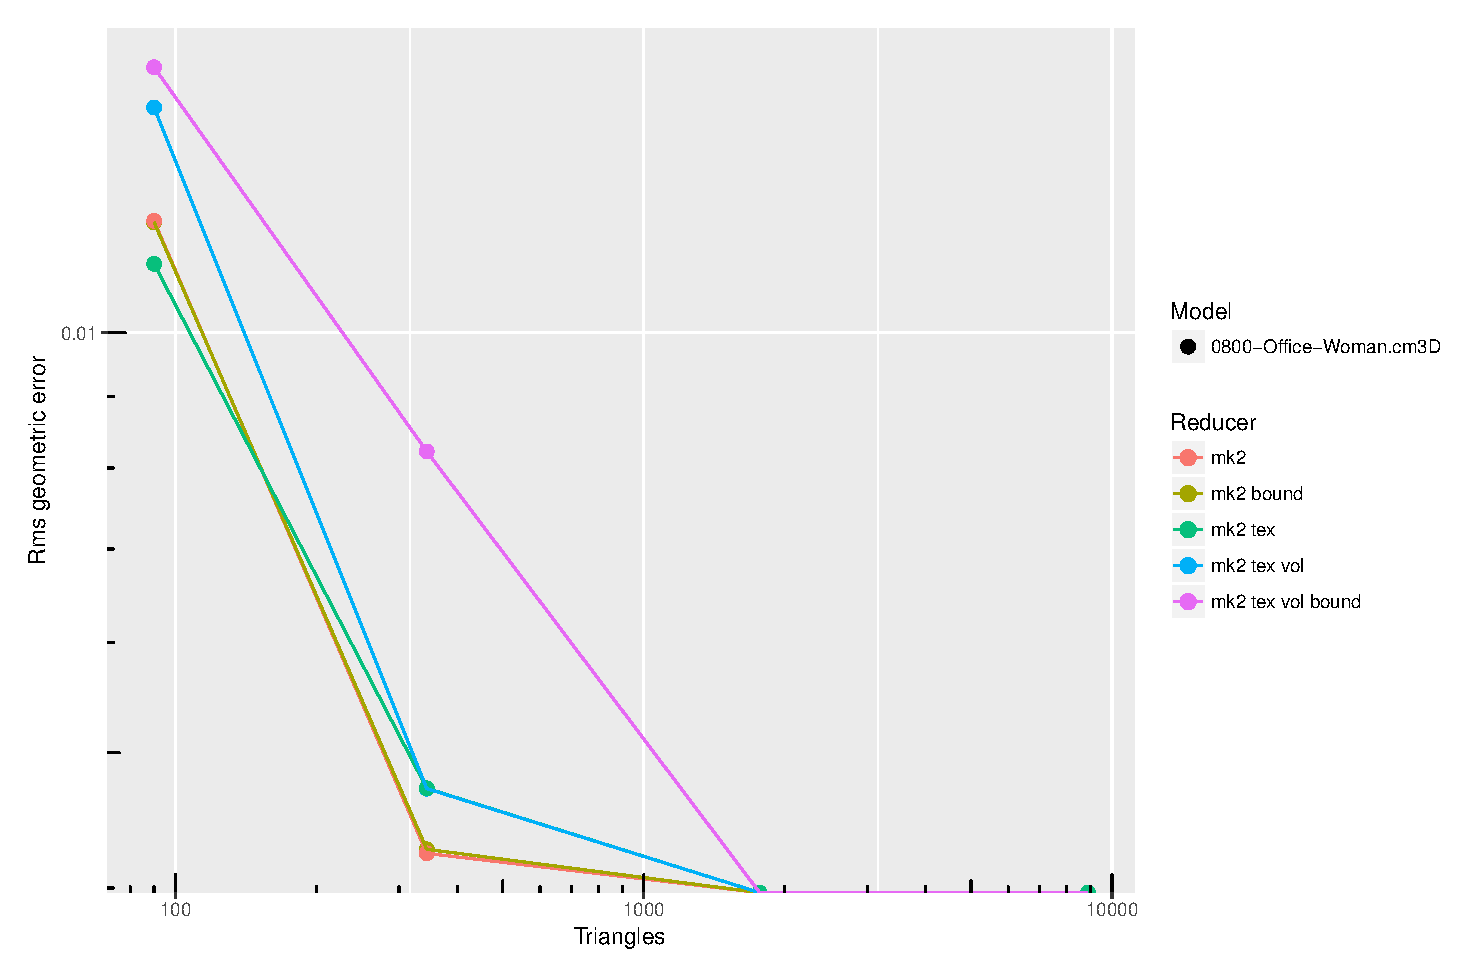
\includegraphics[width=\textwidth]{figures/Rdata/geometric_800.eps}
  \caption{Rms geometric error of ``office woman'' model}
  \label{fig:woman_geometric_error}
\end{figure}


\begin{figure}[ht]
  \centering
  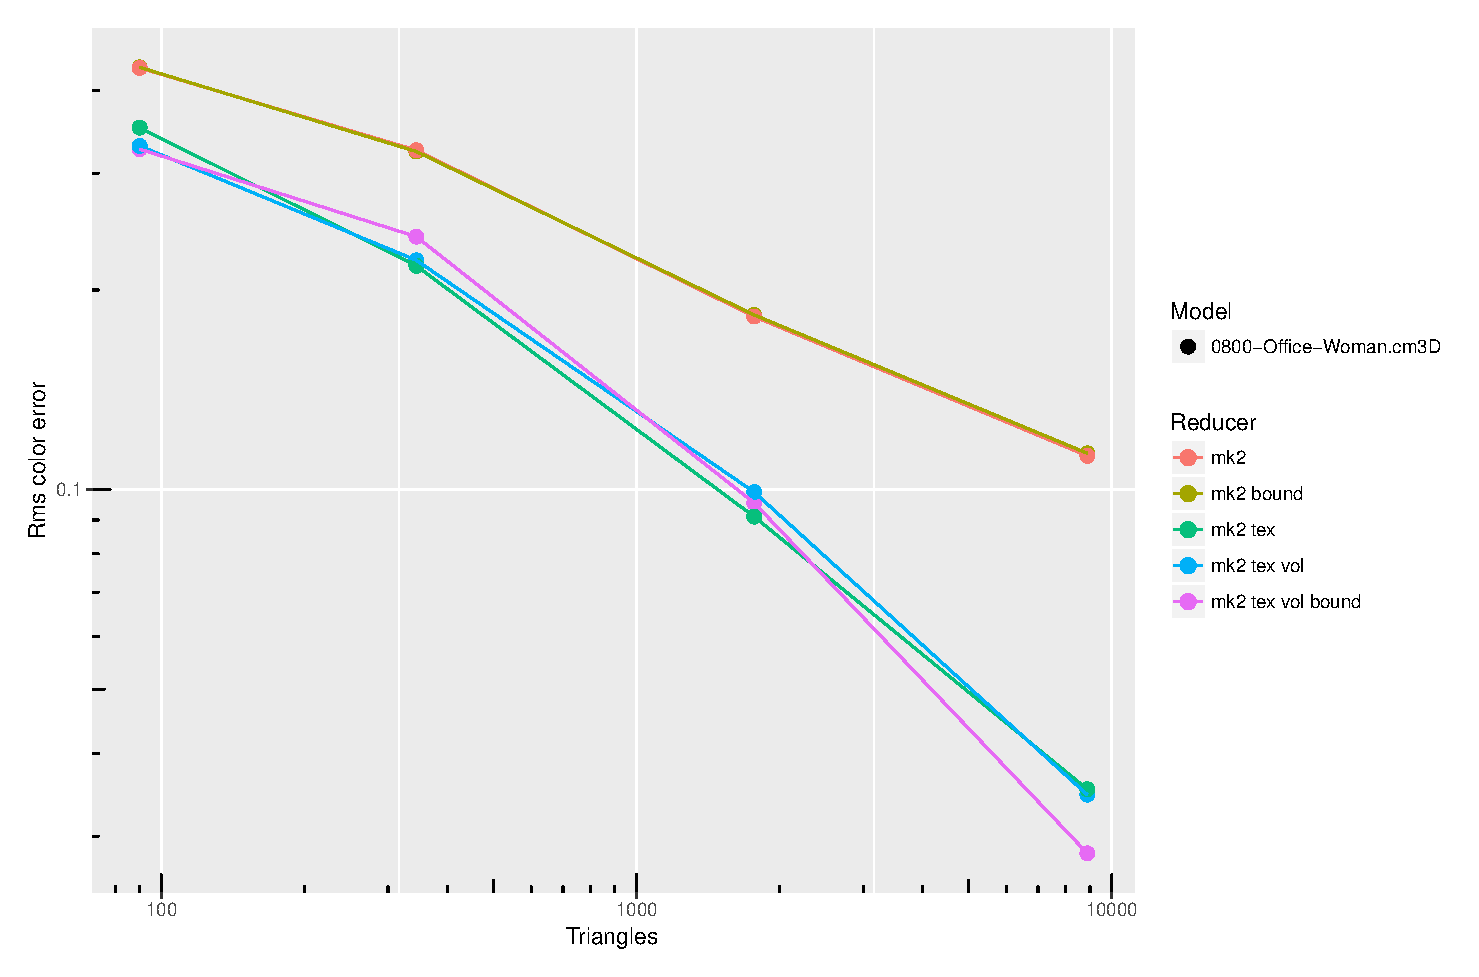
\includegraphics[width=\textwidth]{figures/Rdata/color_800.eps}
  \caption{Rms color error of ``office woman'' model}
  \label{fig:woman_color_error}
\end{figure}
\fi

\section{Luminance error}
RMS luminance error was computed by rendering multiple images of a model from different camera positions as explained in \cref{sec:metrics_for_appearance_preservation} and can be seen in \cref{fig:mean_luminance_error}. Four LoD:s are presented where \emph{super} have the most amount of triangles and \emph{low} have the least amount of triangles. The error was measured for different settings of seam and volume preservation to determine what setting would give the best result. Nine different models with triangle counts between 10000 and 30118 was used in this evaluation. For each model the RMS luminance error was computed for all LoD:s. A mean of the RMS was then obtained and is presented together with a 95\% confidence interval in \cref{fig:mean_luminance_error}.

\begin{figure}[ht]
  \centering
  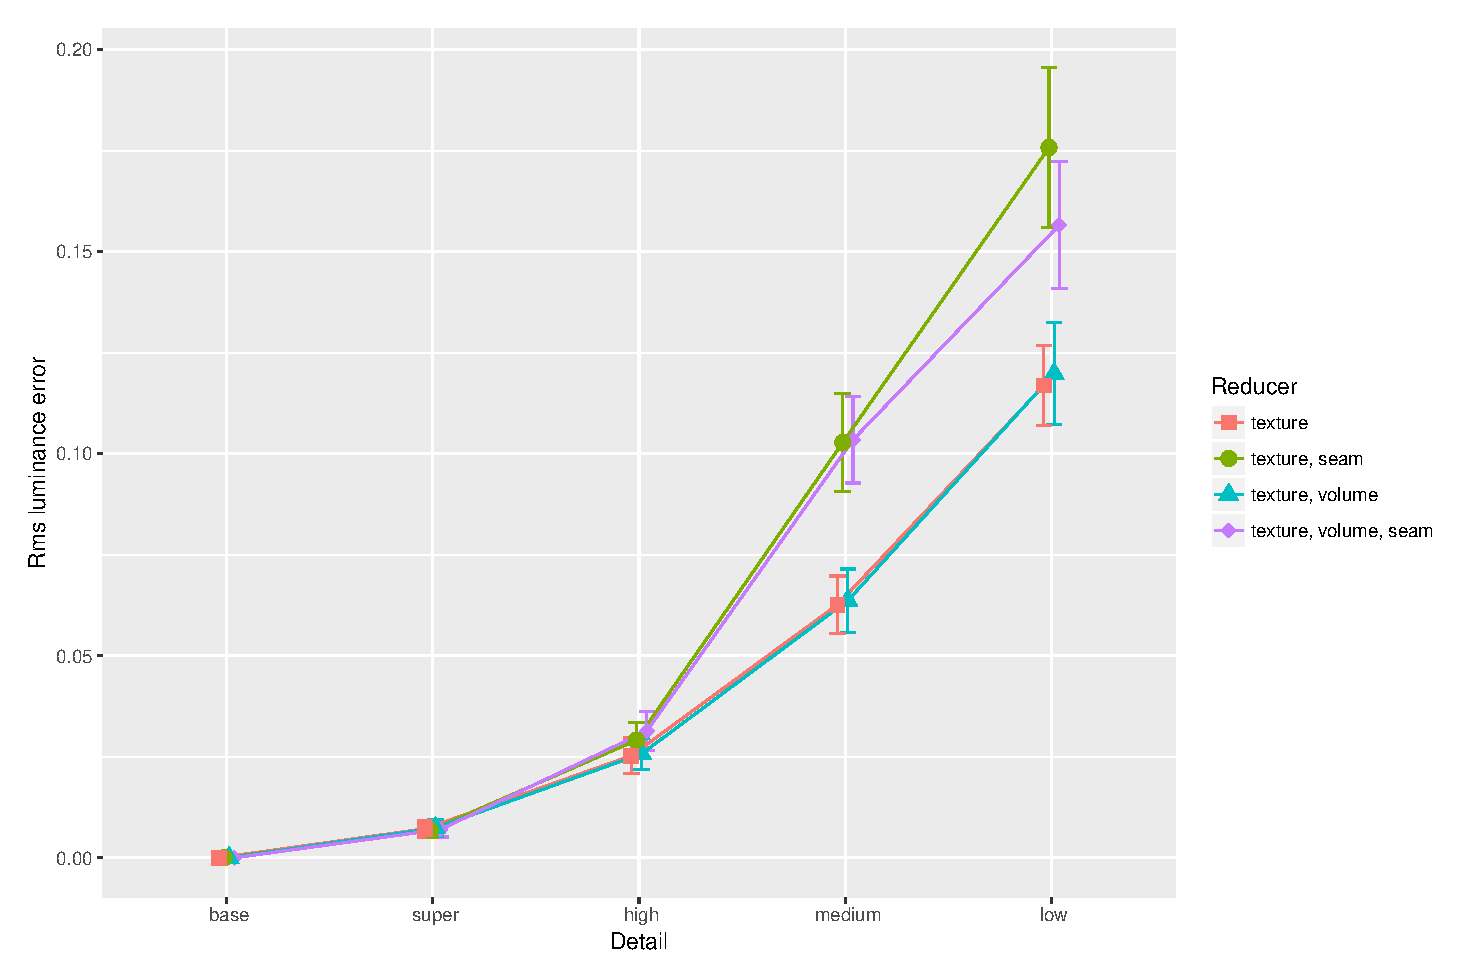
\includegraphics[width=.6\textwidth]{Rdata/rms_luminance.eps}
  \caption{Rms luminance error}
  \label{fig:mean_luminance_error}
\end{figure}

\clearpage



 
\section{Geometric and Color Error}
To see how the geometry and color of a model is affected by simplification, points were sampled on the surface of the simplified mesh and the original mesh. The distances from the sampled points on one mesh to the closest points on the other mesh can then be used to measure the distance between the meshes as well as the color difference. This is described in more detail in \cref{sec:evaluation}. Both the RMS and the maximum error was measured for different settings of seam and volume preservation with the \emph{office woman model} and the values are plotted in \cref{fig:geo_col_error}. Note that the x-axis and y-axis have a logarithmic scale.

\begin{figure}[ht]
  \centering
  \begin{subfigure}[b]{.49\textwidth}
    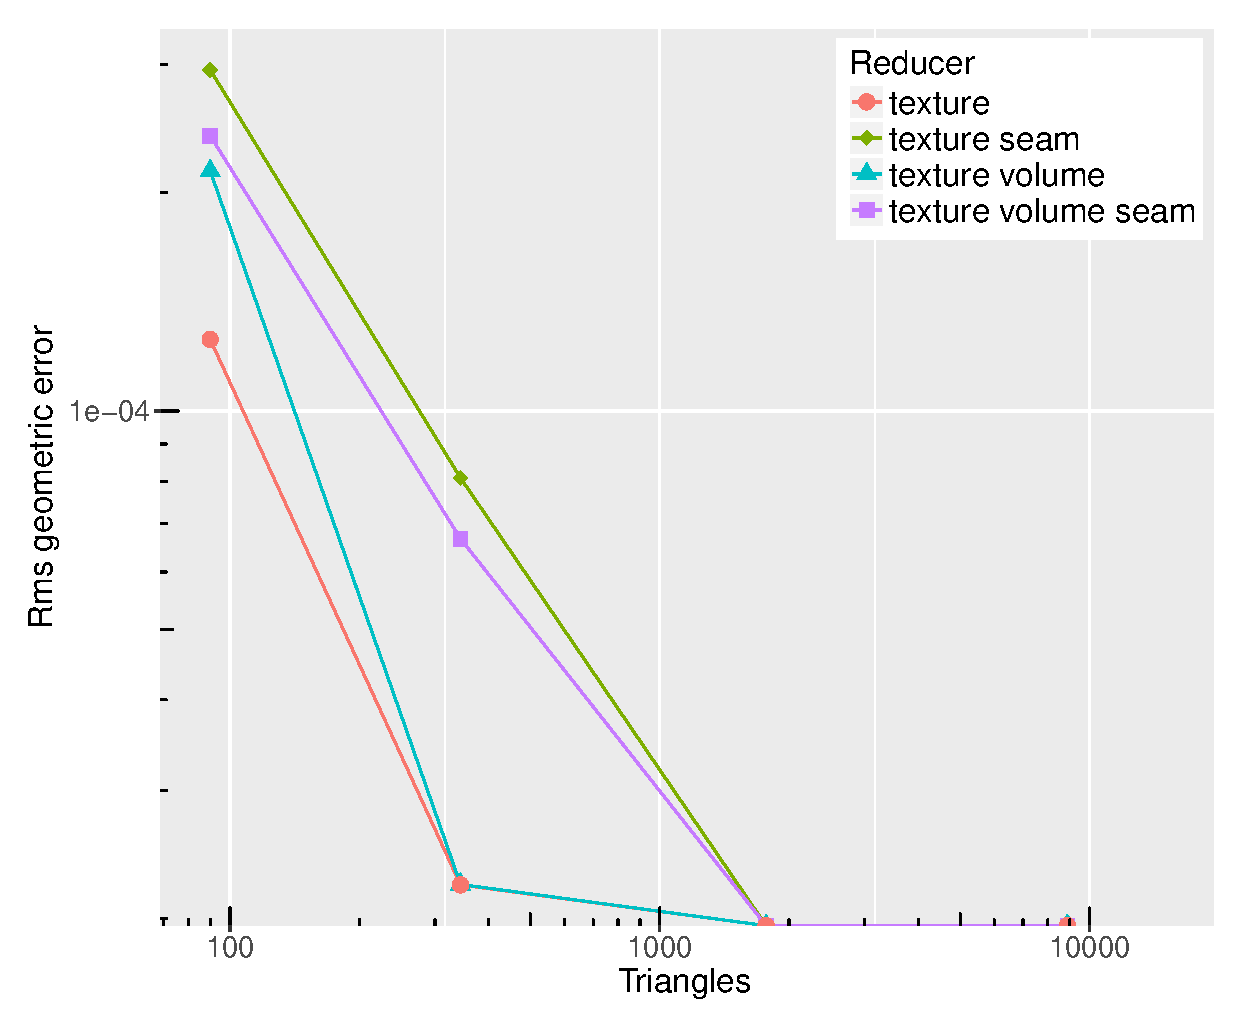
\includegraphics[width=\textwidth]{Rdata/rms_geometric_800.eps}
  \end{subfigure}
  \hfill
  \begin{subfigure}[b]{.49\textwidth}
    \right
    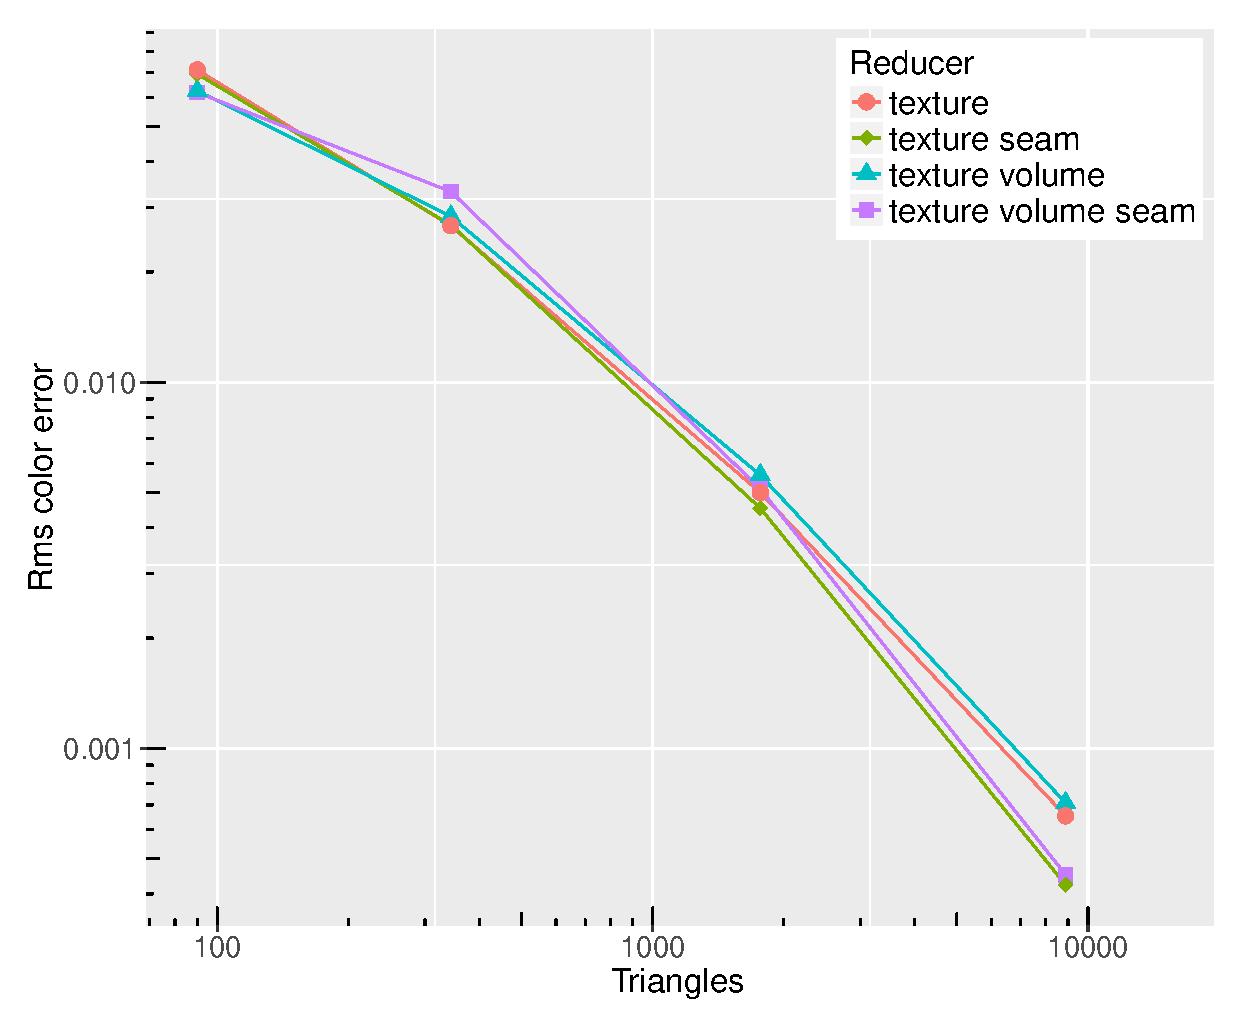
\includegraphics[width=\textwidth]{Rdata/rms_color_800.eps}
  \end{subfigure}

  \begin{subfigure}[b]{.49\textwidth}
    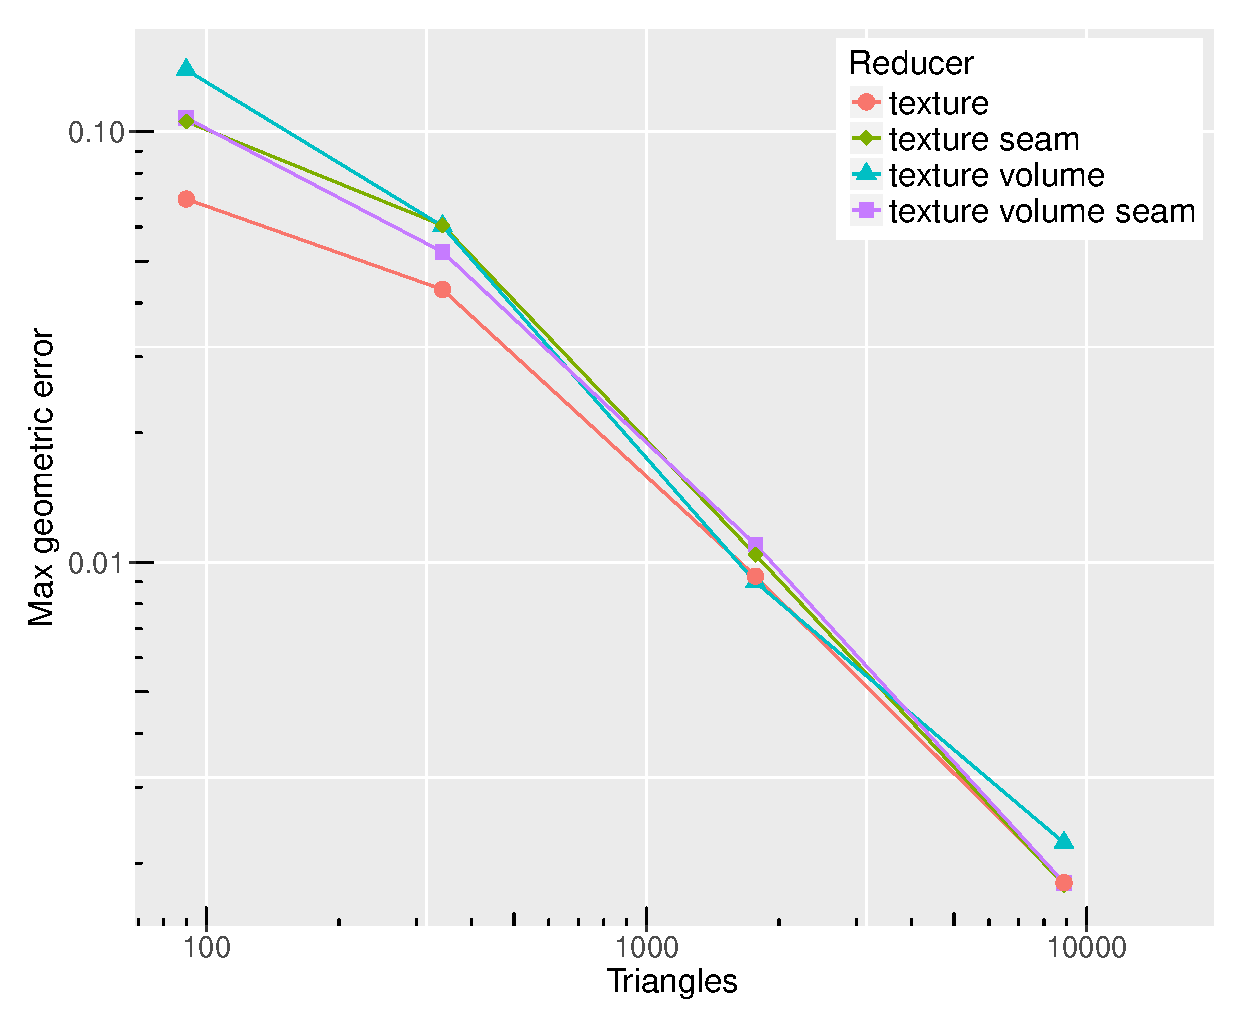
\includegraphics[width=\textwidth]{Rdata/max_geometric_800.eps}
  \end{subfigure}
  \hfill
  \begin{subfigure}[b]{.49\textwidth}
    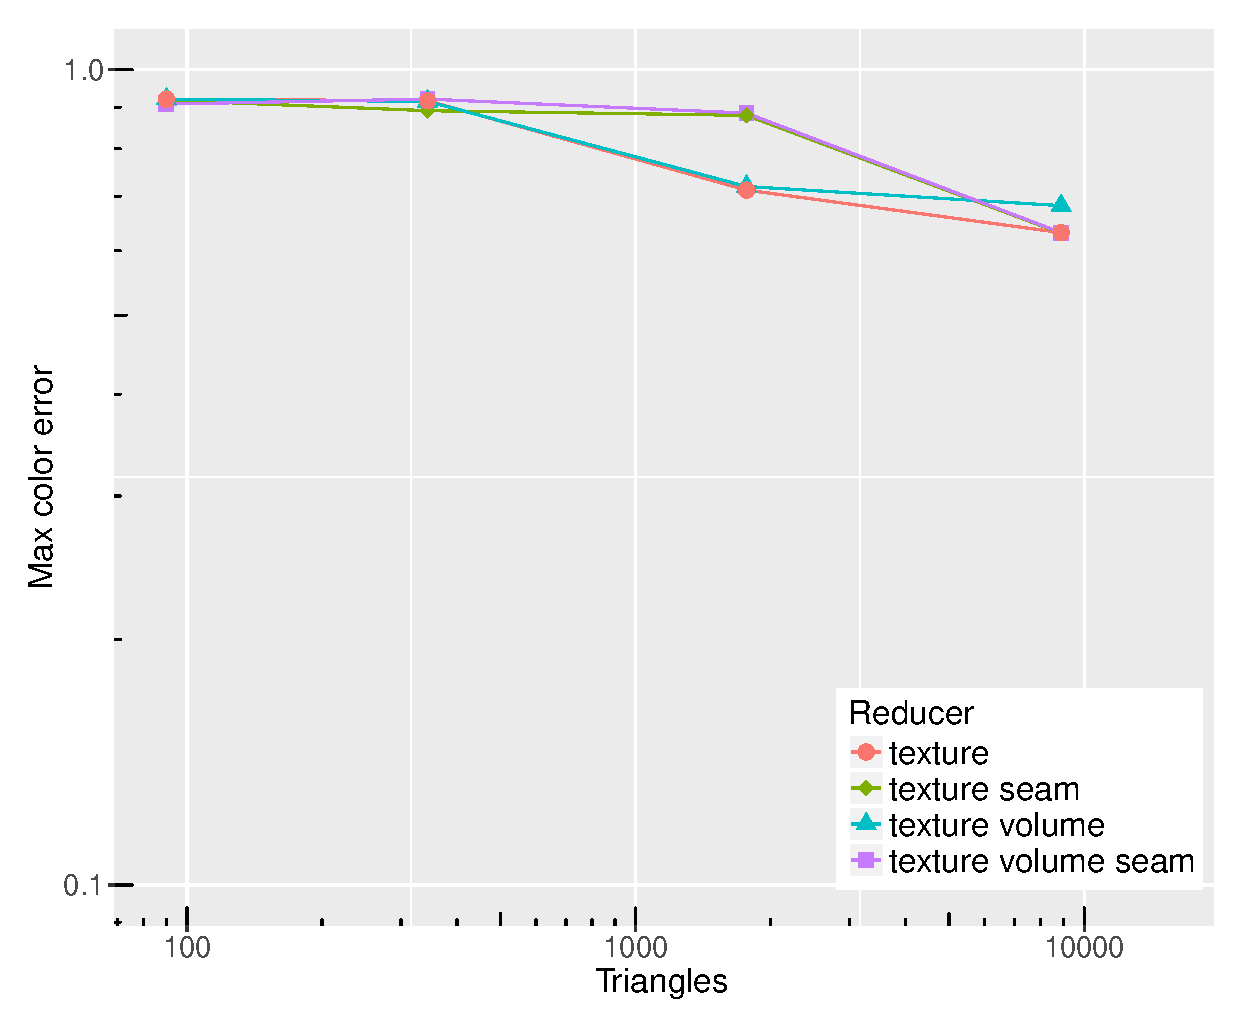
\includegraphics[width=\textwidth]{Rdata/max_color_800.eps}
  \end{subfigure}
  \caption{Office woman geometric and color error}
  \label{fig:geo_col_error}
\end{figure}

\clearpage
        
\section{Volume Preservation}
When simplification is performed the volume of the mesh may be reduced. How much the volume of a simplified mesh differ from the original mesh is therefore plotted in \cref{fig:volume_diff}. Reduction was made with four configurations of texture, volume, and seam considerations for nine models. The mean difference in volume is plotted together with a 95\% confidence interval.

\begin{figure}[ht]
  \centering
  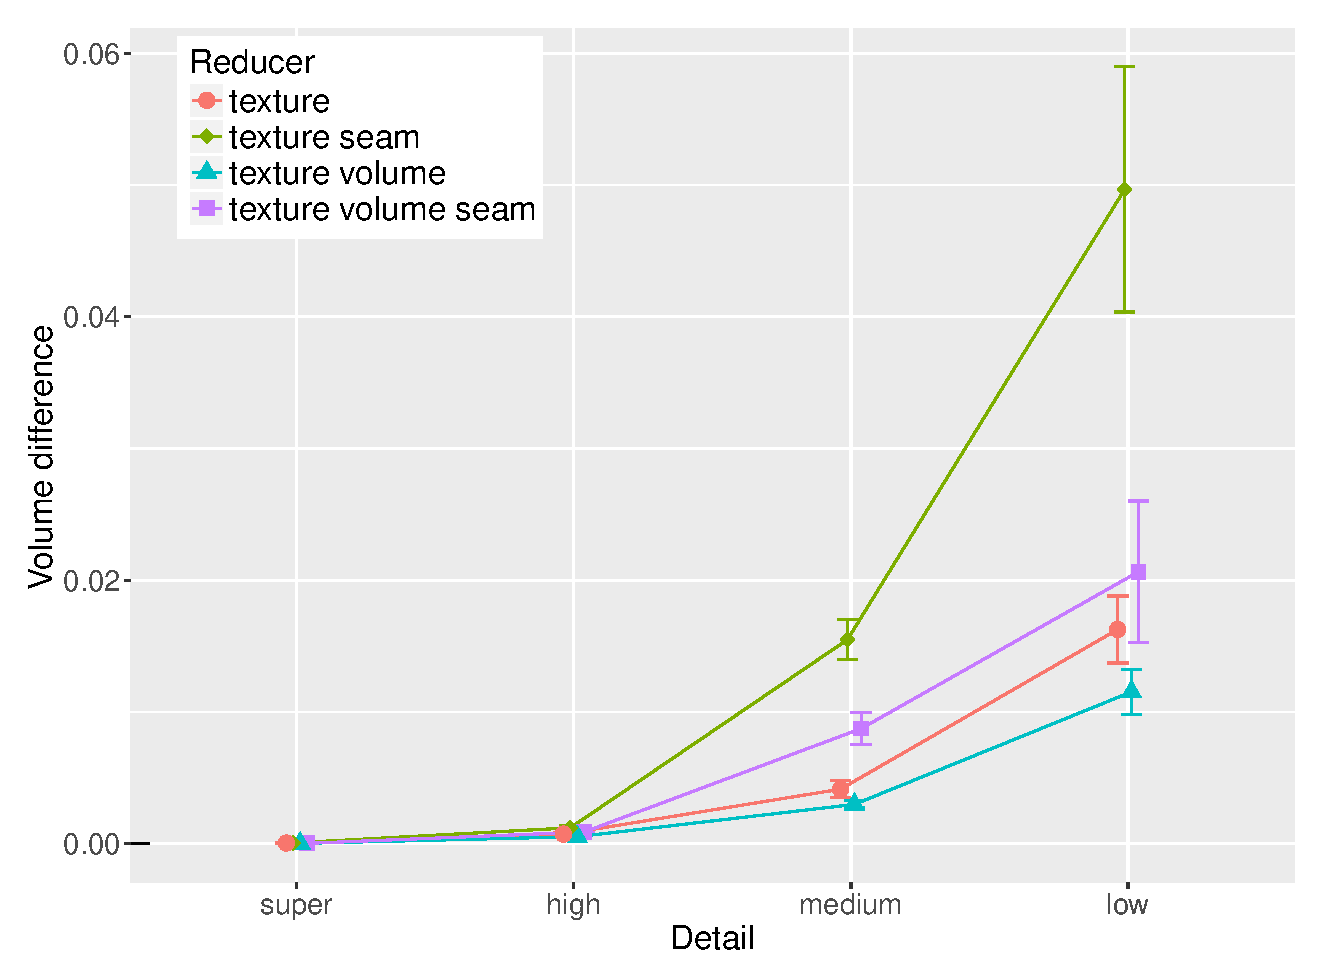
\includegraphics[width=.6\textwidth]{Rdata/volume_diff.eps}
  \caption{Mean difference in volume}
  \label{fig:volume_diff}
\end{figure}

\clearpage

\section{Improved Texture}
A pull-push algorithm was implemented in order to improve the texture that is used by a mesh since undefined areas may be seen when applied to a simplified model. Given a texture (\cref{fig:original_texture_atlas}), rays are casted for each pixel in order to generate a black and white image that distinguish valid pixels from invalid pixels. Valid pixels get a white color and invalid pixels a black color as seen in \cref{fig:valid_pixels}. Pixels with a corresponding black pixel will be filled in by the pull-push algorithm. This will result in the texture seen in \cref{fig:improved_texture} where all the empty pixels have been filled in.

\begin{figure}[ht]
  \centering
  \begin{subfigure}[b]{.3\textwidth} 
    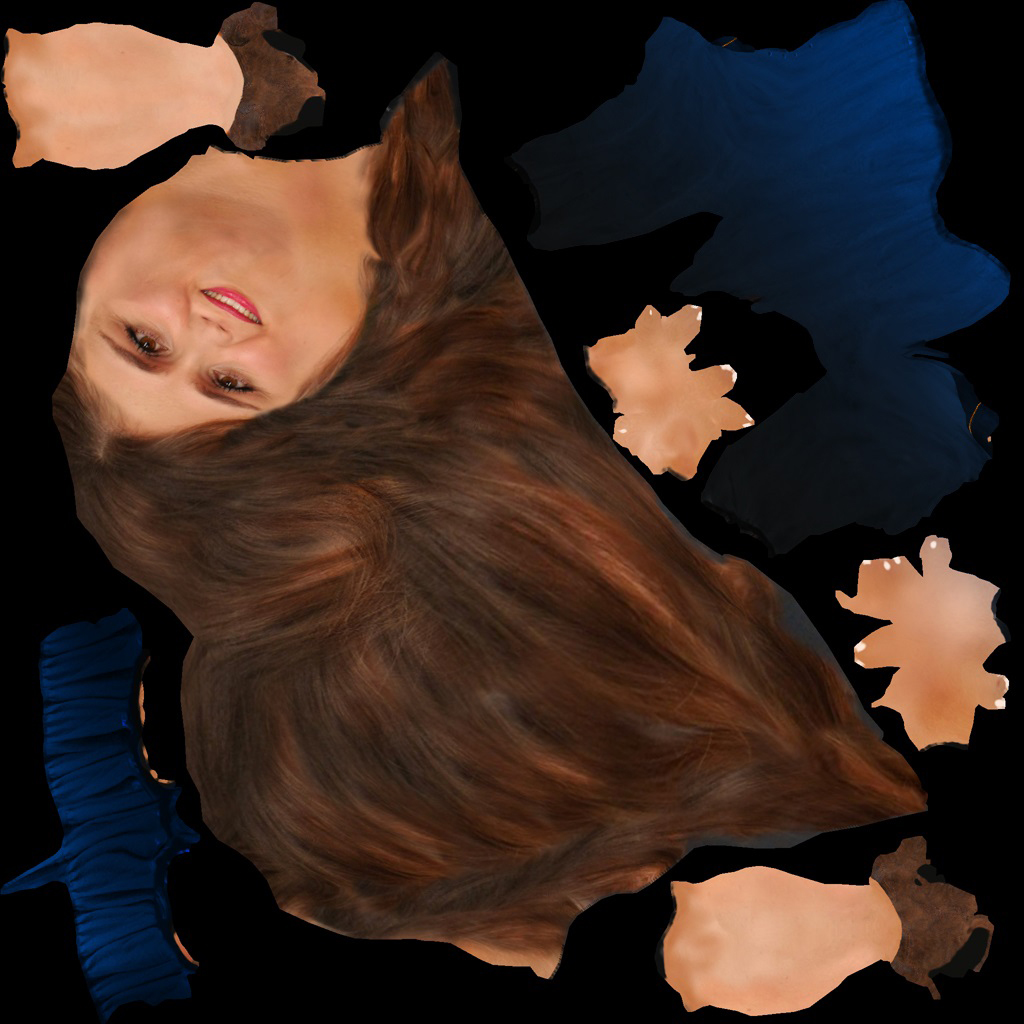
\includegraphics[width=\textwidth]{woman_input.jpg}
    \caption{Original}
    \label{fig:original_texture_atlas}
  \end{subfigure}
  ~
  \begin{subfigure}[b]{.3\textwidth}
    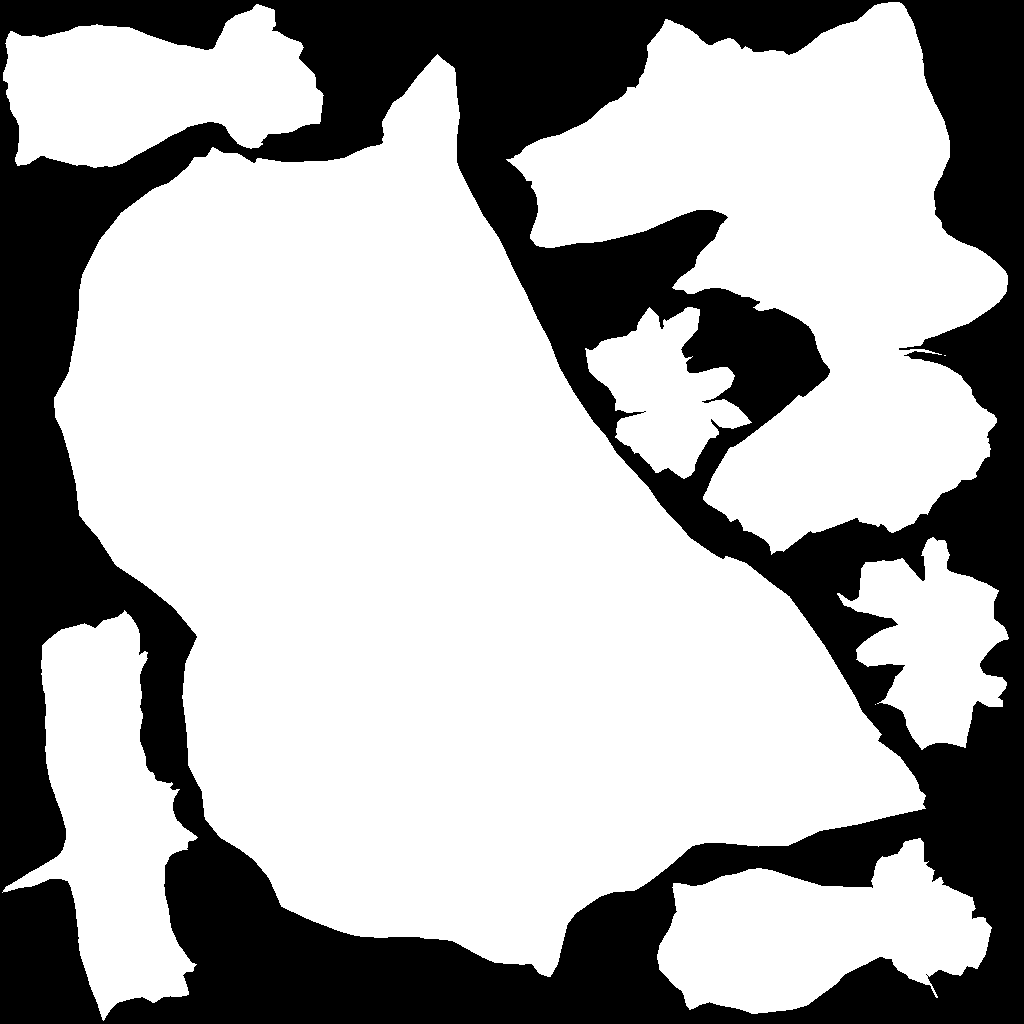
\includegraphics[width=\textwidth]{woman_bound.png}
    \caption{Valid pixels}
    \label{fig:valid_pixels}
  \end{subfigure}
  ~
  \begin{subfigure}[b]{.3\textwidth}
    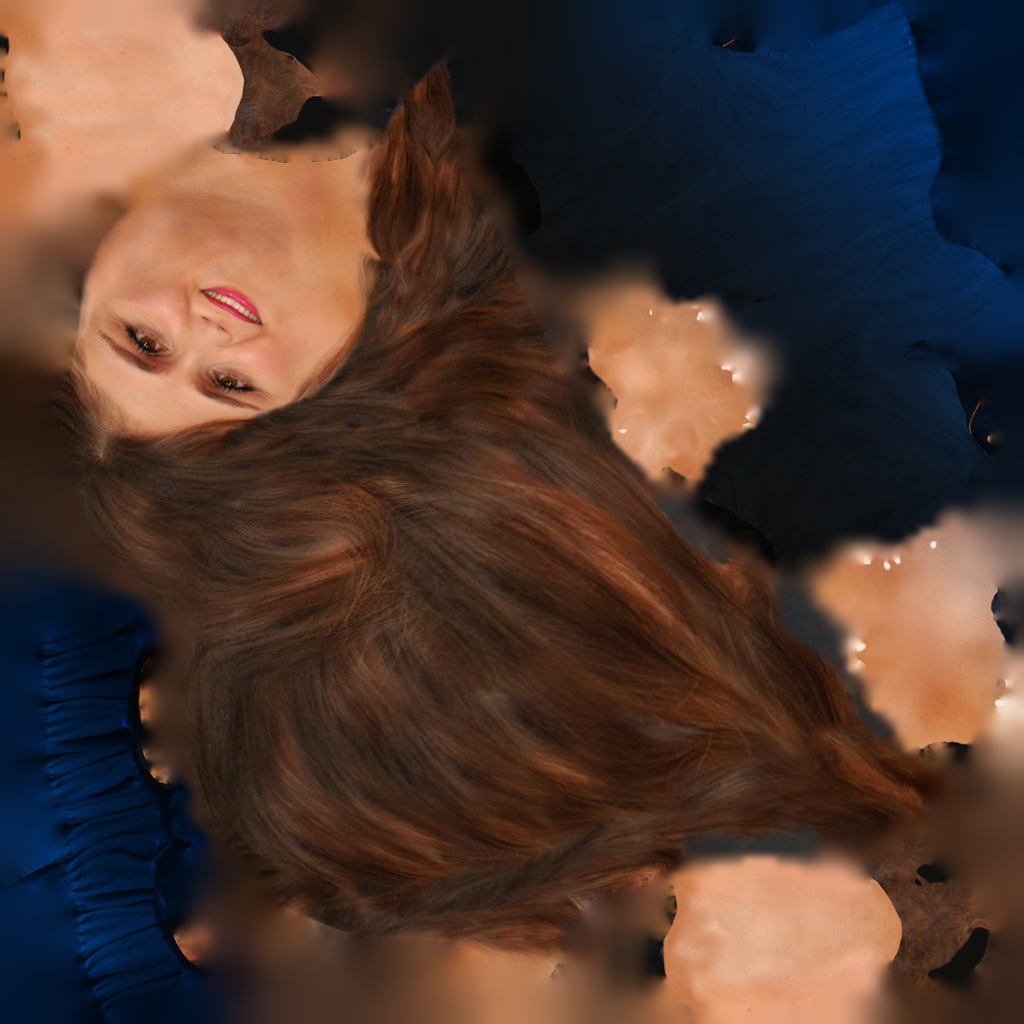
\includegraphics[width=\textwidth]{woman_output.png}
    \caption{Improved texture}
    \label{fig:improved_texture}
  \end{subfigure}
  \caption{Filling in empty pixels in the texture atlas}
  \label{fig:improve_texture_atlas}
\end{figure}

Simplification of the office woman model introduced black areas on the legs where the original seam used to be (\cref{fig:using_original_texture}). Trying to improve the appearance by applying the new improved texture results in the model shown in \cref{fig:using_improved_texture}.

\begin{figure}[ht]
  \centering
  \begin{subfigure}[b]{.15\textwidth}
    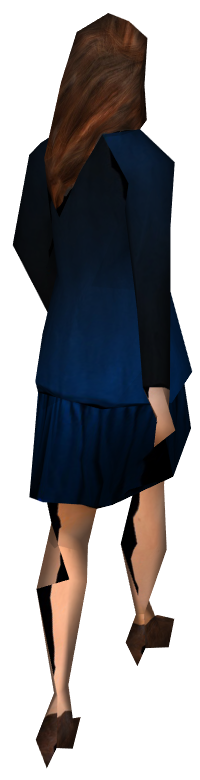
\includegraphics[width=\textwidth]{woman_render.png}
    \caption{Using original texture}
    \label{fig:using_original_texture}
  \end{subfigure}
  \qquad
  \begin{subfigure}[b]{.15\textwidth}
    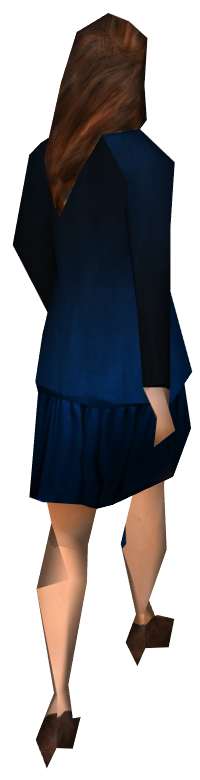
\includegraphics[width=\textwidth]{woman_render_improved.png}
    \caption{Using improved texture}
    \label{fig:using_improved_texture}
  \end{subfigure}
  \caption{Comparison between original and improved texture}
  \label{fig:texture_comparison}
\end{figure}

\clearpage

% base:   14996
% super:   8886
% high:    1768
% medium:   344
% low:       90
\section{Comparison of LoD:s}

To compare how different LoD:s are affected by the simplification the office woman model have been rendered after simplification. The original model has 14996 triangles and the LoD:s super, high, medium, and low have 8886, 1768, 344, 90 triangles respectively. Renderings of the Lod:s have been created both with equal distance from the camera and with the camera placed at the distance where they would actually be used which can be seen in \cref{fig:woman_lodeq,fig:woman_lod} respectively. When creating these LoD:s with the simplification algorithm the seam and volume was not considered, only the texture.

\begin{figure}[ht]
  \centering
  \begin{subfigure}[b]{.22\textwidth}
    \includegraphics[width=\textwidth]{woman/equal_distance/1.png}
    \caption{super}
    \label{fig:womaneq0}
  \end{subfigure}
  \begin{subfigure}[b]{.22\textwidth}
    \includegraphics[width=\textwidth]{woman/equal_distance/2.png}
    \caption{high}
    \label{fig:womaneq1}
  \end{subfigure}
  \centering
  \begin{subfigure}[b]{.22\textwidth}
    \includegraphics[width=\textwidth]{woman/equal_distance/3.png}
    \caption{medium}
    \label{fig:womaneq2}
  \end{subfigure}
  \begin{subfigure}[b]{.22\textwidth}
    
\includegraphics[width=\textwidth]{woman/equal_distance/4.png}
    \caption{low}
    \label{fig:womaneq3}
  \end{subfigure}
  \caption{Office woman LoD:s at equal distance}
  \label{fig:woman_lodeq}
\end{figure}

\begin{figure}[ht]
  \centering
  \begin{subfigure}[b]{.22\textwidth}
    \includegraphics[width=\textwidth]{woman/cropped/1.png}
    \caption{super}
    \label{fig:woman0}
  \end{subfigure}
  \begin{subfigure}[b]{.22\textwidth}
    \includegraphics[width=\textwidth]{woman/cropped/2.png}
    \caption{high}
    \label{fig:woman1}
  \end{subfigure}
  \centering
  \begin{subfigure}[b]{.22\textwidth}
    \includegraphics[width=\textwidth]{woman/cropped/3.png} 
    \caption{medium}
    \label{fig:woman2}
  \end{subfigure}
  \begin{subfigure}[b]{.22\textwidth}
    
\includegraphics[width=\textwidth]{woman/cropped/4.png}
    \caption{low}
    \label{fig:woman3}
  \end{subfigure}
  \caption{Office woman LoD:s at their corresponding distance} 
  \label{fig:woman_lod}
\end{figure}
